\documentclass[12pt,letterpaper,landscape]{article}
\usepackage{amsmath}
\usepackage{amsfonts}
\usepackage{amssymb}
\usepackage{graphicx}
\usepackage[left=2cm,right=2cm,top=2cm,bottom=2cm]{geometry}
\usepackage{hyperref}
\usepackage{caption}
\usepackage{subcaption}
	\captionsetup{font=small,
				  labelfont=bf,
				  labelsep=period}

%%%%%%%%%%%%%%%%%%%%%%%%%%%%%% User specified LaTeX commands.
\newcommand*{\bs}[1]{\boldsymbol{#1}}

%%%%%%%%%%%%%%%%%%%%%%%%%%%%%% Title

\title{\textbf{Information for simulations in Wave Propagation}}
\author{Nicol\'as Guar\'in-Zapata}
\date{\today}


%%%%%%%%%%%%%%%%%%%%%%%%%%%%%% Document
\begin{document}
\maketitle

\section{Consistent units}
Although is a good practice to convert the equations to their dimensionless versions, we still need to plug numbers into our numerical algorithm. For that aim, we need to use consistent units, as presented in the following table.
\begin{table}[h]
\centering
\begin{tabular}{|c|c|c|c|c|}
\hline 
\textbf{Quantity} & \textbf{SI} & \textbf{SI (mm)} & \textbf{US (ft)} & \textbf{US (inch)} \\ 
\hline 
Length & m & mm & ft & in \\ 
\hline 
Force & N & N & lbf & lbf \\ 
\hline 
Mass & kg & tonne (10$^3$ kg) & slug & lbf s$^2$/in \\ 
\hline 
Time & s & s & s & s \\ 
\hline 
Stress & Pa (N/m$^2$) & MPa (N/mm$^2$) & lbf/ft$^2$ & psi (lbf/in$^2$) \\ 
\hline 
Energy & J & mJ (10$^{-3}$) & ft lbf & in lbf \\ 
\hline 
Density & kg/m$^3$ & tonne/mm$^3$ & slug/ft$^3$ & lbf s$^2$/in$^4$ \\ 
\hline 
\end{tabular}
\end{table} 

\section{Relations between elastic constants}
\begin{table}[h]
\centering %
\begin{tabular}{|c|c|c|c|c|c|c|c|c|c|c|}
\hline 
 & $\bs{(K,E)}$  & $\bs{(K,\lambda)}$  & $\bs{(K,G)}$  & $\bs{(K,\nu)}$  & $\bs{(E,G)}$  & $\bs{(E,\nu)}$  & $\bs{(\nu,G)}$  & $\bs{(\nu,\lambda)}$  & $\bs{(G,\lambda)}$  & $\bs{(G,M)}$ \\
\hline 
$\bs{K}=$  & $K$  & $K$  & $K$  & $K$  & $\frac{EG}{3(3G-E)}$  & $\frac{E}{3(1-2\nu)}$  & $\lambda+\frac{2G}{3}$  & $\frac{\lambda(1+\nu)}{3(1-2\nu)}$  & $\frac{2G(1+\nu)}{3(1-2\nu)}$  & $M-\frac{4G}{3}$ \\
\hline 
$\bs{E}=$  & $E$  & $\frac{9K(K-\lambda)}{3K-\lambda}$  & $\frac{9KG}{2K+G}$  & $3K(1-2\nu)$  & $E$  & $E$  & $\frac{G(3\lambda+2G)}{\lambda+G}$  & $\frac{\lambda(1+\nu)(1-2\nu)}{\nu}$  & $2G(1+\nu)$  & $\frac{G(3-M-4G)}{M-2G}$ \\
\hline 
$\bs{\lambda}=$  & $\frac{3K(3KE)}{9K-E}$  & $\lambda$  & $K-\frac{2G}{3}$  & $\frac{3K\nu}{1+\nu}$  & $\frac{G(E-2G)}{EG-E}$  & $\frac{E\nu}{(1+\nu)(1-2\nu)}$  & $\lambda$  & $\lambda$  & $\frac{2G\nu}{1-2\nu}$  & $M-2G$ \\
\hline 
$\bs{G}=$  & $\frac{3KE}{9K-E}$  & $\frac{3(K-\lambda)}{2}$  & $G$  & $\frac{3K(1-2\nu)}{2(1+\nu)}$  & $G$  & $\frac{E}{2(1+\nu)}$  & $G$  & $\frac{\lambda(1-2\nu)}{2\nu}$  & $G$  & $G$ \\
\hline 
$\bs{\nu}=$  & $\frac{3K-E}{6K}$  & $\frac{\lambda}{3K-\lambda}$  & $\frac{3K-2G}{2(3K+G)}$  & $\nu$  & $\frac{E}{2G}-1$  & $\nu$  & $\frac{\lambda}{2(\lambda+G)}$  & $\nu$  & $\nu$  & $\frac{M-2G}{2(M-G)}$ \\
\hline 
$\bs{M}=$  & $\frac{3K(3K+E)}{9K-E}$  & $3K-2\lambda$  & $K+\frac{4G}{3}$  & $\frac{3K(1-\nu)}{1+\nu}$  & $\frac{G(4G-E)}{3G-E}$  & $\frac{E(1-\nu)}{(1+\nu)(1-2\nu)}$  & $\lambda+2G$  & $\frac{\lambda(1-\nu)}{\nu}$  & $\frac{2G(1-\nu)}{1-2\nu}$  & $M$ \\
\hline 
\end{tabular}
\end{table}


$K$: Bulk modulus, $\lambda$: Lam\'e's first parameter, $E$: Young's
modulus, $G$: Shear modulus, $\nu$: Poisson's ratio, $M$: P-wave
modulus.


\section{Relations for elastic wave speeds}

The P-wave is a dilatational wave with speed $\alpha$ given by 
\begin{align*}
 & \alpha^{2}=\frac{\lambda+2G}{\rho},\qquad\alpha^{2}=\frac{G(1-\nu)}{\rho},\\
 & \alpha^{2}=\frac{M}{\rho},\qquad\alpha^{2}=\frac{E(1-\nu)}{(1+\nu)(1-2\nu)\rho},\\
 & \alpha^{2}=\frac{2\beta^{2}(1-\nu)}{1-2\nu}.
\end{align*}
 The S-wave is a distorsional wave with speed $\beta$ given by 
\begin{align*}
 & \beta^{2}=\frac{G}{\rho}\\
 & \beta^{2}=\frac{E}{2(1+\nu)\rho},\\
 & \beta^{2}=\frac{\alpha^{2}(1-2\nu)}{2(1-\nu)}.
\end{align*}
 Some particular values for the ratio 
\[
\frac{\alpha^{2}}{\beta^{2}}=\frac{2(1-\nu)}{1-2\nu}
\]
 are 
\begin{align*}
 & \frac{\alpha^{2}}{\beta^{2}}=\frac{4}{3}\quad\mbox{for }\nu=-1\enspace,\\
 & \frac{\alpha^{2}}{\beta^{2}}=2\quad\mbox{for }\nu=0\enspace,\\
 & \frac{\alpha^{2}}{\beta^{2}}=4\quad\mbox{for }\nu=\frac{1}{3}\enspace,\\
 & \frac{\alpha^{2}}{\beta^{2}}\rightarrow\infty\quad\mbox{when }\nu\rightarrow\frac{1}{2}\enspace.
\end{align*}

\begin{figure}[h]
\centering
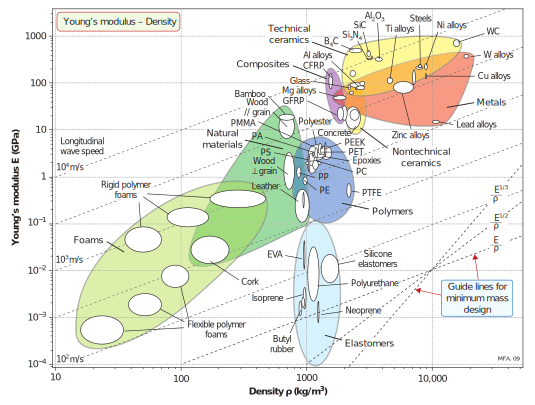
\includegraphics[width=0.8\textwidth]{img/E_vs_density-vector.pdf} 
\caption{Ashby chart for Young Modulus vs density. The lines show the sound speed, that is the speed for a wave in a rod made of this material and is between the longitudinal and shear wave speeds --for Poisson ratios in (-0.5,0.5). Taken from \emph{Ashby, Michael F. ``Materials selection in mechanical design." MRS BULLETIN 30 (2005): 995.}}
\end{figure}

\section{Courant-Friedrichs-Lewy condition}

The Courant-Friedrichs-Lewy condition (CFL condition) is a necessary condition for convergence while solving certain partial differential equations (usually hyperbolic PDEs) numerically by the method of finite differences. It arises when explicit time-marching schemes are used for the numerical solution. The condition is named after Richard Courant, Kurt Friedrichs, and Hans Lewy who described it in their 1928 paper
\cite{CFL}.

The criterion could be stated as 
\begin{align*}
C=v_{x}\frac{\Delta t}{\Delta x}\leq C_{max}\qquad\mbox{in 1D}\enspace;\\
C=v_{x}\frac{\Delta t}{\Delta x}+v_{y}\frac{\Delta t}{\Delta y}\leq C_{max}\qquad\mbox{in 2D}\enspace;\\
C=v_{x}\frac{\Delta t}{\Delta x}+v_{y}\frac{\Delta t}{\Delta y}+v_{z}\frac{\Delta t}{\Delta z}\leq C_{max}\qquad\mbox{in 3D}\enspace;
\end{align*}
 Where $v_{x_{i}}$ is the phase speed (for wave phenomena) in the $x_{i}$ direction, $\Delta x_{i}$ is the minimum spatial discretization in $x_{i}$ direction, $\Delta t$ is the time step and $C_{max}$ is the maximum allowable value for $C$, which depends on the time discretization scheme but should be less than 1.

In the case of elastodynamics and for a spatial discretization with
the finite element method, the criterion could be re-stated as 
\begin{align*}
C\leq\alpha\frac{\Delta t}{h}\leq C_{max}\qquad\mbox{in 1D}\enspace;\\
C\leq2\alpha\frac{\Delta t}{h}\leq C_{max}\qquad\mbox{in 2D}\enspace;\\
C\leq3\alpha\frac{\Delta t}{h}\leq C_{max}\qquad\mbox{in 3D}\enspace;
\end{align*}
where $\alpha$ is the phase speed for the P-wave and $h$ is the
minimum distance between consecutive nodes. This give us the maximum
allowable timestep as 
\begin{align}
\Delta t\leq C_{max}\frac{h}{\alpha}\qquad\mbox{in 1D}\enspace;\\
\Delta t\leq\frac{C_{max}}{2}\frac{h}{\alpha}\qquad\mbox{in 2D}\enspace;\\
\Delta t\leq\frac{C_{max}}{3}\frac{h}{\alpha}\qquad\mbox{in 3D}\enspace.
\end{align}
A graphical representation of the criterion is given in Figure \ref{fig:CFL}. Intuitively, we can think about the CFL condition as a limit in the speed for transferring information from one node to its neighbors; this \emph{speed} should be less than the speed for propagation of phenomena in the wave.
\begin{figure}[h]
\centering
\includegraphics[width=0.7\textwidth]{img/CFLcondition.png}
\caption{Graphic representation of the CFL condition in 1D. \textit{L.A. Barba et al. Practical Numerical Methods with Python, 2014.}}\label{fig:CFL}
\end{figure}


\section{Nyquist criterion}

The Nyquist–Shannon sampling theorem (also Nyquist-Shannon-Whittaker theorem), after Harry Nyquist and Claude Shannon, in the literature more commonly referred to as the Nyquist sampling theorem or simply as the sampling theorem, is a fundamental result in the field of information theory, in particular telecommunications and signal processing. Sampling is the process of converting a signal (for example, a function of continuous time or space) into a numeric
sequence (a function of discrete time or space). Shannon's version of the theorem states \cite{Shannon}:
\begin{quote}
If a function $x(t)$ contains no frequencies higher than $B$ hertz,
it is completely determined by giving its ordinates at a series of
points spaced $1/(2B)$ seconds apart. 
\end{quote}
This theorem implies for us in the numerical simulation of wave propagation
that 
\[
h\leq\frac{\lambda}{2}\enspace,
\]
 where $h$ is the maximum distance between consecutive nodes and
$\lambda$ is the shortest wavelength that want to be sampled. So,
the selection of $h$ is commonly 
\[
h=\frac{\lambda}{k}\enspace,
\]
 where $k>2$ is a factor that depends on the numerical method. For
finite element methods $k$ is commonly 10, and for spectral element
methods $k$ is reduced to 5 \cite{Komatitsch99}.


\section{Information for different pulse signals}
In wave propagation problems we must work with time signals that are finite in time, let's say wave pulses (or wave packets in the Quantum Mechanics jargon). Some times we are interested in wave pulses because they are useful as wavefronts representation. Furthermore, wave packets are important since we cannot store information in a wave with a single frequency\footnote{That's why phase speed of waves can be higher than speed of light. For non-dissipative media, the energy (and so the information) travel with the group velocity \cite{book:Brillouin1}.}. There is a trade off between the localization in time (duration of the pulse) and frequency (concentration of the energy around a specific value). This fact is well discussed in Quantum Mechanics texts since it re ects the discussion about wave{particle duality and uncertainty principle \cite{book:Zetilli}. When we have finite time signals its corresponding Fourier transform will be in the whole frequency domain. In general terms, while more concentrated in the time domain, more spread in the frequency domain. From a numerical point of view we need to truncate the maximum frequency allowed for our simulations.

In the following \emph{subsections} we exposed some truncation tips for different wave pulses. This is important because numerically we cannot consider the complete spectrum of a pulse, since normally they cover the whole frequency domain. We will refer to the function in time as $f(t)$, and to its Fourier transform as $\hat{f}(\omega)$. Since the ``energy" carried for the wave per frequency is proportional to the square of the absolute value of the Fourier transform $\hat{f}^2(\omega)$, we can compare the energy in the frequency interval $[0,\omega_{\max}]$ to the energy content in $[0,\infty)$\footnote{We just need to compute one halfspace because the other half has the same values.}. Thus, as a figure of merit we define
\begin{equation}
R(\omega_{\max}) = \frac{\int\limits_{0}^{\omega_{\max}} \hat{f}^2 (\omega)\ \rm{d}\omega}{\int\limits_{0}^{\infty} \hat{f}^2 (\omega)\ \rm{d}\omega}\times 100\% \enspace ,
\label{eq:trunc_energy}
\end{equation}
and tell us the proportion of energy taken into account if we neglect circular frequencies higher than $\omega_{\max}$.

\subsection{Ricker wavelet}
It is common to use a Ricker wavelet as the input signal in simulations since it has the energy concentrated around a circular frequency $\omega_{c}$. Let's write the signal as 
\[f(t)=\left(\frac{12t^{2}}{b^{2}}-1\right)e^{-\frac{6t^{2}}{b^{2}}}\enspace,\]
 where $b$ is the elapsed time between the peaks in the time domain \cite{Papageorgiou91}. The Fourier transform for this signal is  
\[\hat{f}(\omega)=-\frac{\sqrt{\pi}b^{3}\omega^{2}e^{-\frac{b^{2}\omega^{2}}{24}}}{2\ 6^{3/2}}\enspace, \]
with a characteristic\footnote{The characteristic frequency is the value at which the peak appears.} circular frequency 
\[\omega_{c}=\frac{2\sqrt{6}}{b}. \]
To satisfy the sampling theorem we need to design our simulations
thinking about the shortest wavelength, so we need to think about
the maximum frequency. To know where to trunk the signal (in the frequency domain) we could compute how much energy is in $[0,\omega_{max}]$ and compare this value with the energy stored in the interval $[0,\infty)$. Some particular values are : 
\begin{align*}
 & R(1.0\omega_{c})=45.06\%\enspace;\\
 & R(1.5\omega_{c})=89.09\%\enspace;\\
 & R(2.0\omega_{c})=99.32\%\enspace;\\
 & R(3.0\omega_{c})=99.99\%\enspace;\\
 & R(4.0\omega_{c})=100.00\%\enspace.
\end{align*}
This can be depicted in
\begin{figure}[h]
    \centering
    \begin{subfigure}[b]{0.45\textwidth}
        \includegraphics[width=\textwidth]{img/ricker_area=1.pdf}
        \caption{Are under the curve in $[0,\omega_c]$.}
    \end{subfigure}\
    %
    \begin{subfigure}[b]{0.45\textwidth}
        \includegraphics[width=\textwidth]{img/ricker_area=2.pdf}
        \caption{Are under the curve in $[0,2\omega_c]$.}
    \end{subfigure}\\
    %
    \begin{subfigure}[b]{0.45\textwidth}
        \includegraphics[width=\textwidth]{img/ricker_area=3.pdf}
        \caption{Are under the curve in $[0,3\omega_c]$.}
    \end{subfigure}
    %
    \begin{subfigure}[b]{0.45\textwidth}
        \includegraphics[width=\textwidth]{img/ricker_area=4.pdf}
        \caption{Are under the curve in $[0,4\omega_c]$.}
    \end{subfigure}
    \caption{Energy distribution in the spectrum of the Ricker wavelet.}
    \label{fig:ricker-areas}
\end{figure}

\begin{thebibliography}{1}
\bibitem{book:Brillouin1} Brillouin, Le\'on, and Arnold Sommerfeld. Wave propagation and group velocity. Vol. 960. New York: Academic Press, 1960.

\bibitem{CFL} Courant, R.; Friedrichs, K.; Lewy, H. (1928), \emph{\"Uber die partiellen Differenzengleichungen der mathematischen Physik} (in German), Mathematische Annalen 100 (1): 32--74.

\bibitem{Shannon} C. E. Shannon, \emph{Communication in the presence of noise}, Proc. Institute of Radio Engineers, vol. 37, no. 1, pp. 10--21, Jan. 1949. Reprint as classic paper in: Proc. IEEE, vol. 86, no. 2, (Feb. 1998).

\bibitem{Komatitsch99} D. Komatitsch and J. Tromp,\emph{Introduction to the spectral element method for three-dimensional seismic wave propagation}, Geophysical Journal International, 1999, (139): 806--822.

\bibitem{Papageorgiou91} A. Papageorgiou and J. Kim,\emph{Stufy of the propagation and amplification of seismic waves in Caracas Valley with reference to the 29 July 1967 earthquake: SH waves}, Bulletin of the Seismological Society of America, 1991, 81 (6): 2214--2233. 

\bibitem{book:Zetilli} Nouredine Zettili. Quantum mechanics: concepts and applications. Wiley, 2009. 

\end{thebibliography}


\end{document}